\documentclass[12pt]{beamer}
\usetheme{Warsaw}
\usepackage[utf8]{inputenc}
\usepackage{amsmath}
\usepackage{amsfonts}
\usepackage{amssymb}
\usepackage{graphicx}
%\author{}
%\title{}
%\setbeamercovered{transparent} 
%\setbeamertemplate{navigation symbols}{} 
%\logo{} 
%\institute{} 
%\date{} 
%\subject{} 
\begin{document}

%\begin{frame}
%\titlepage
%\end{frame}

%\begin{frame}
%\tableofcontents
%\end{frame}

\begin{frame}{Versuchsziel}
\begin{itemize}
\item Bestimmung der Schallgeschwindigkeit und des Elastizitätsmoduls in Metallen durch Messung der Schallfrequenz
\item (dünner) Metallstab wird durch Anschlag zu longitudinalen Schwingungen angeregt 
\end{itemize}
\end{frame}

\begin{frame}{Aufbau}
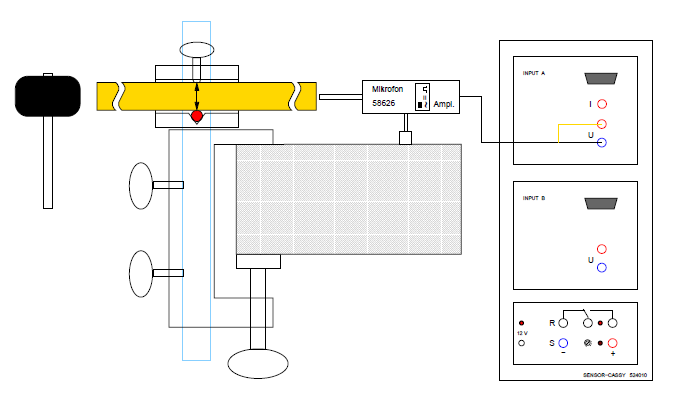
\includegraphics[width=\linewidth,height=\textheight,keepaspectratio]{Bilder/AufbauMessungSchallgeschwindigkeitMetallstab.PNG}
\centering
\end{frame}

\begin{frame}{Durchführung}
\begin{itemize}
\item Mikrofon im Amplitudenmodus
\item CASSY-Eistellungen
\begin{itemize}
\item kleines Abtastinervall($50\mu s$)
\item 16000 Messungen
\item mittlerer Messbereich($-3V\leq U\leq 3V$)
\end{itemize}
\item Messwerte
\begin{itemize}
\item Länge: Einfachmessung mit $\sigma_{stat}\approx0.3mm$ und $\sigma_{sys}=0.56mm$
\item Dicke, Masse, Frequenz werden durch Mehrfachmessung bestimmt
\end{itemize}
\end{itemize}
\end{frame}

\begin{frame}{Auswertung}
\begin{itemize}
\item Elastizitätsmodul:
\begin{equation}
E = 16 f_0^2 \cdot \dfrac{L M}{\pi D^2}
\end{equation}
\item Geschwindigkeit:
\begin{equation}
v_l = \lambda_0 \cdot f_0 = 2\cdot L \cdot f_0
\end{equation}

\item Auswertung der Messergebnisse durch eine Fast-Fourier-Transformation
\end{itemize}
\end{frame}

\begin{frame}{Fourieranalysen}
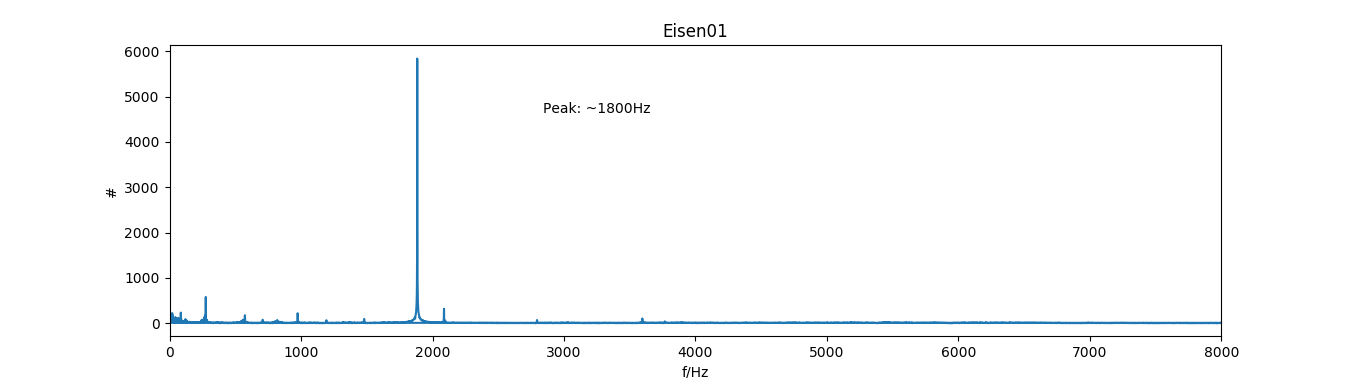
\includegraphics[width=0.5\textwidth, height=0.4\textheight]{Bilder/Eisen01_fourier.png}
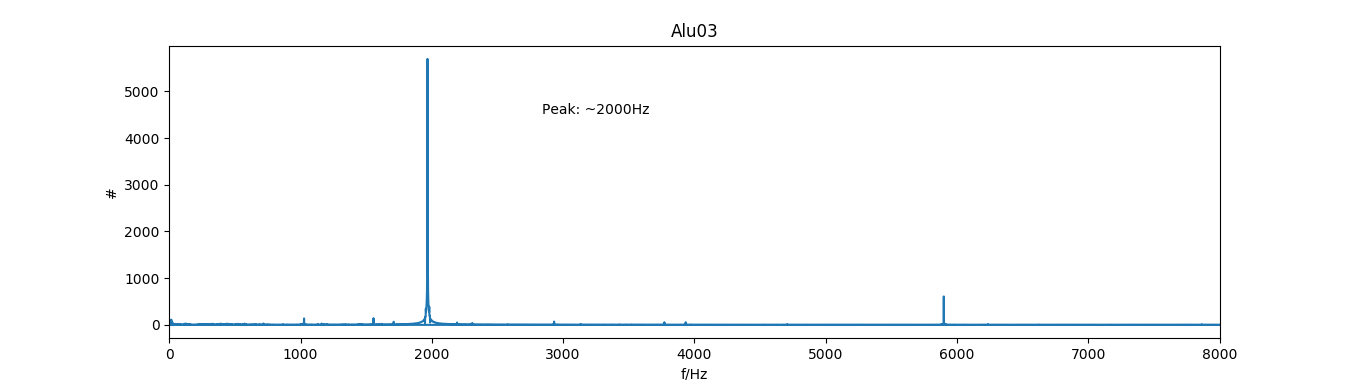
\includegraphics[width=0.5\linewidth,height=0.4\textheight]{Bilder/Alu03_fourier.png}\\
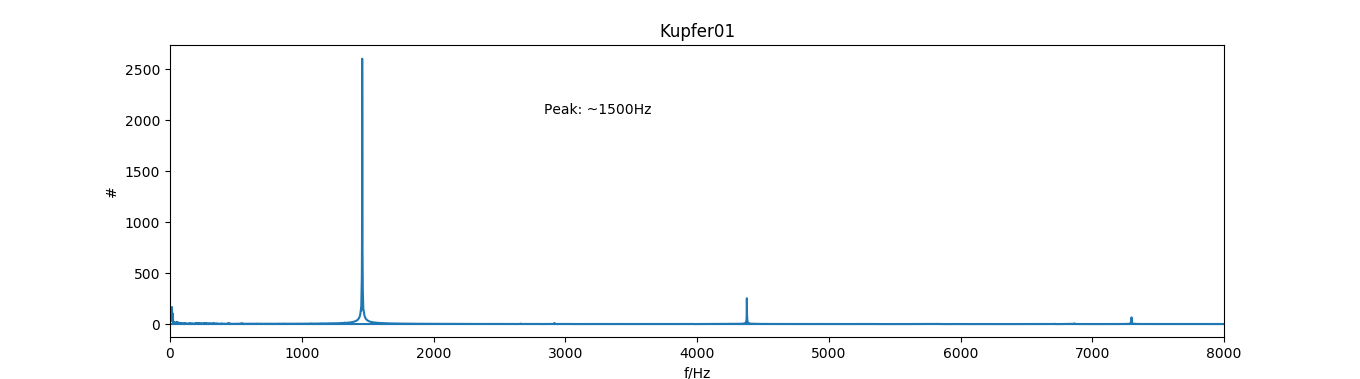
\includegraphics[width=0.5\linewidth,height=0.4\textheight]{Bilder/Kupfer01_fourier.png}
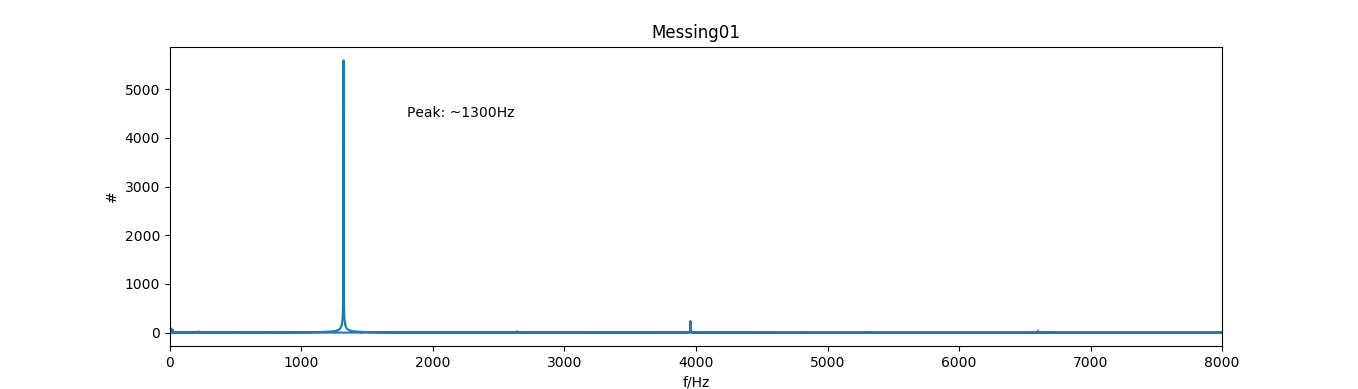
\includegraphics[width=0.5\linewidth,height=0.4\textheight]{Bilder/Messing01_fourier.png}\\
\end{frame}

\begin{frame}{Messergebnisse}
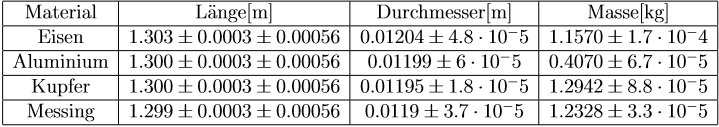
\includegraphics[width=\linewidth,height=\textheight,keepaspectratio]{Bilder/Material_Metalle.PNG}\\
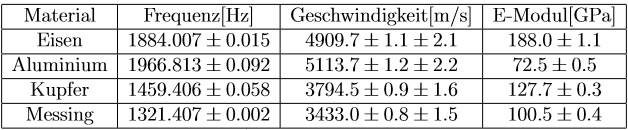
\includegraphics[width=\linewidth,height=\textheight,keepaspectratio]{Bilder/Ergebnisse_Metall.PNG}
\end{frame}

\begin{frame}{Vergleich mit Literaturwerten}
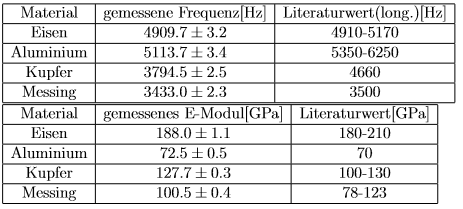
\includegraphics[width=\linewidth,height=\textheight,keepaspectratio]{Bilder/Literaturwerte_Metalle.PNG}\\
\begin{itemize}
\item Fazit:
\begin{itemize}
\item Ergebnisse sind sinnvoll
\item Abweichungen durch ungenaue Materialeigenschaften
\end{itemize}
\end{itemize}
\end{frame}
\end{document}